\begin{figure}[htbp]
\section*{ NF1}
\centering
\begin{subfigure}[b]{0.5\textwidth}
\centering
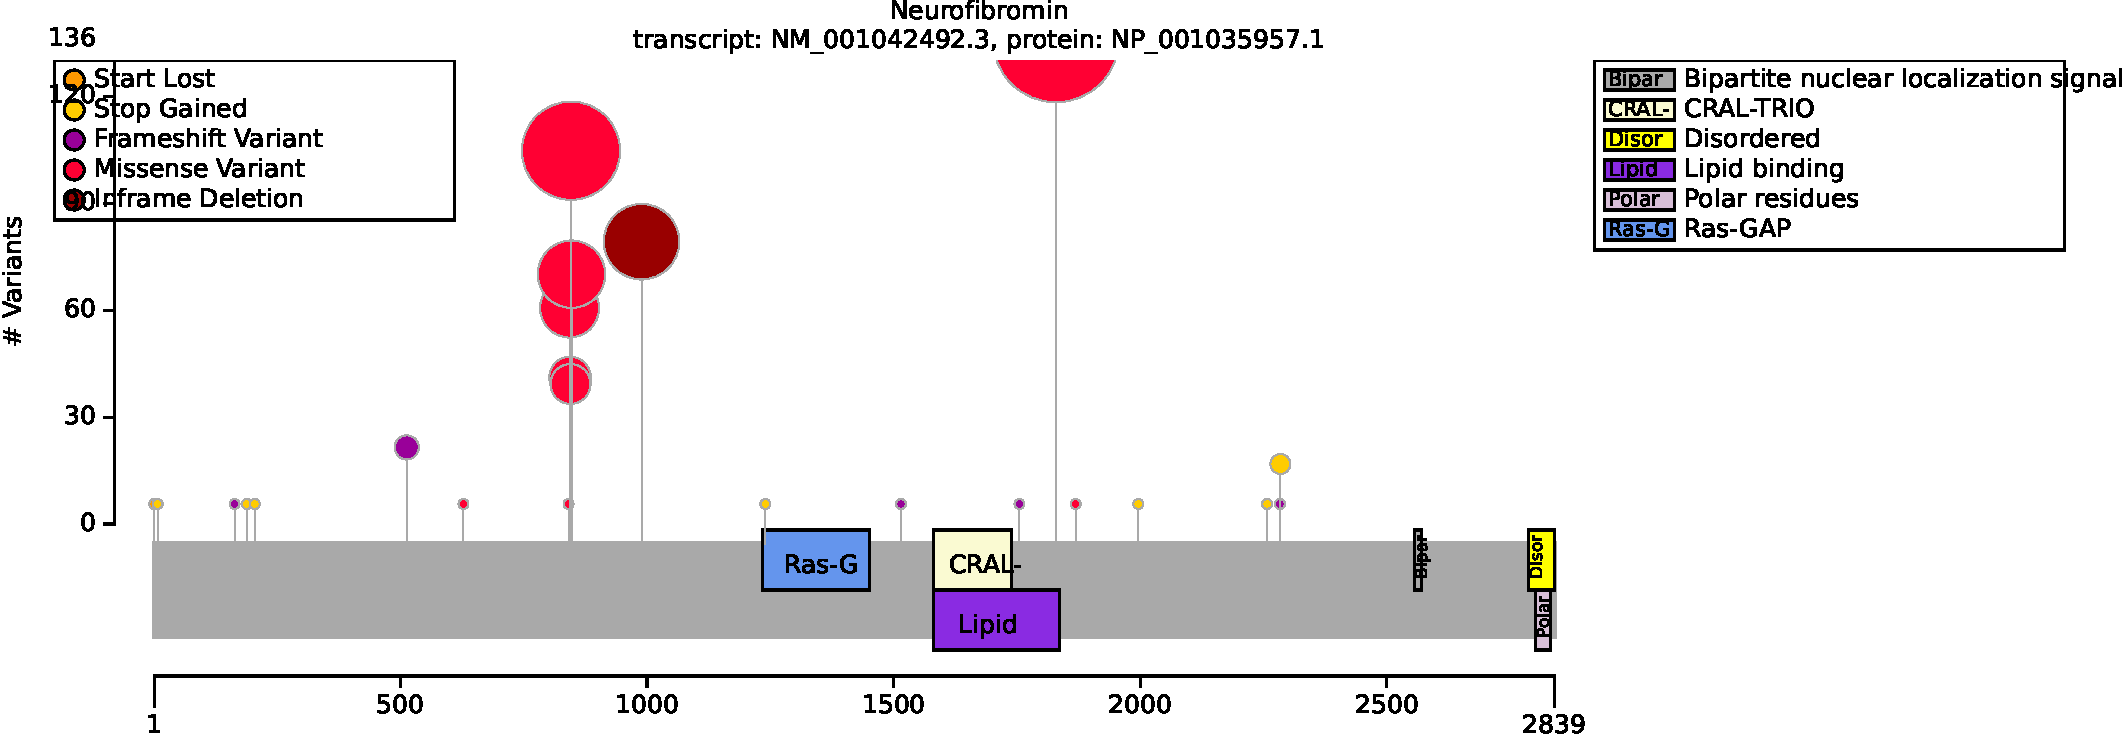
\includegraphics[width=\textwidth]{ img/NF1_protein_diagram.pdf} 
\captionsetup{justification=raggedright,singlelinecheck=false}
\caption{Distribution of variants in NF1}
\end{subfigure}


\begin{subfigure}[b]{0.95\textwidth}
\centering
\resizebox{\textwidth}{!}{
\begin{tabular}{llllrr}
\toprule
HPO term & p.Arg1830 & other & p-value & adj. p-value\\
\midrule
Axillary freckling [HP:0000997] & 20/79 (25\%) & 105/175 (60\%) & $3.66\times 10^{-7}$ & $2.01\times 10^{-6}$\\
Freckling [HP:0001480] & 76/133 (57\%) & 201/222 (91\%) & $6.28\times 10^{-13}$ & $6.91\times 10^{-12}$\\
Plexiform neurofibroma [HP:0009732] & 0/135 (0\%) & 68/260 (26\%) & $1.71\times 10^{-14}$ & $3.76\times 10^{-13}$\\
Neurofibroma [HP:0001067] & 5/8 (62\%) & 153/162 (94\%) & 0.012 & 0.030\\
Scoliosis [HP:0002650] & 8/125 (6\%) & 48/240 (20\%) & $4.02\times 10^{-4}$ & 0.001\\
Lisch nodules [HP:0009737] & 11/91 (12\%) & 72/193 (37\%) & $6.58\times 10^{-6}$ & $2.90\times 10^{-5}$\\
Inguinal freckling [HP:0030052] & 8/79 (10\%) & 84/170 (49\%) & $4.86\times 10^{-10}$ & $3.56\times 10^{-9}$\\
Pulmonic stenosis [HP:0001642] & 13/105 (12\%) & 5/162 (3\%) & 0.005 & 0.013\\
Optic nerve glioma [HP:0009734] & 0/39 (0\%) & 39/137 (28\%) & $1.71\times 10^{-5}$ & $6.28\times 10^{-5}$\\
\bottomrule
\end{tabular}
}
\captionsetup{justification=raggedright,singlelinecheck=false}
\caption{         Fisher Exact Test performed to compare HPO annotation frequency with respect to p.Arg1830 and other. Total of
        22 tests were performed. }
\end{subfigure}

\begin{subfigure}[b]{0.95\textwidth}
\centering
\resizebox{\textwidth}{!}{
\begin{tabular}{llllrr}
\toprule
HPO term & Met992del & other & p-value & adj. p-value\\
\midrule
Axillary freckling [HP:0000997] & 0/14 (0\%) & 125/240 (52\%) & $8.57\times 10^{-5}$ & 0.001\\
Plexiform neurofibroma [HP:0009732] & 0/44 (0\%) & 68/351 (19\%) & $2.05\times 10^{-4}$ & 0.001\\
Lisch nodules [HP:0009737] & 3/36 (8\%) & 80/248 (32\%) & 0.003 & 0.008\\
Inguinal freckling [HP:0030052] & 0/14 (0\%) & 92/235 (39\%) & 0.003 & 0.008\\
Lipoma [HP:0012032] & 5/44 (11\%) & 4/284 (1\%) & 0.003 & 0.008\\
\bottomrule
\end{tabular}
}
\captionsetup{justification=raggedright,singlelinecheck=false}
\caption{         Fisher Exact Test performed to compare HPO annotation frequency with respect to Met992del and other. Total of
        13 tests were performed. }
\end{subfigure}

\begin{subfigure}[b]{0.95\textwidth}
\centering
\resizebox{\textwidth}{!}{
\begin{tabular}{llllrr}
\toprule
HPO term & Leu847Pro & other & p-value & adj. p-value\\
\midrule
Axillary freckling [HP:0000997] & 50/61 (82\%) & 75/193 (39\%) & $3.55\times 10^{-9}$ & $7.81\times 10^{-8}$\\
Freckling [HP:0001480] & 54/54 (100\%) & 223/301 (74\%) & $5.30\times 10^{-7}$ & $5.83\times 10^{-6}$\\
Plexiform neurofibroma [HP:0009732] & 24/66 (36\%) & 44/329 (13\%) & $4.63\times 10^{-5}$ & $3.39\times 10^{-4}$\\
Lisch nodules [HP:0009737] & 22/42 (52\%) & 61/242 (25\%) & $7.48\times 10^{-4}$ & 0.003\\
Inguinal freckling [HP:0030052] & 34/60 (57\%) & 58/189 (31\%) & $3.92\times 10^{-4}$ & 0.002\\
Optic nerve glioma [HP:0009734] & 15/33 (45\%) & 24/143 (17\%) & $8.57\times 10^{-4}$ & 0.003\\
\bottomrule
\end{tabular}
}
\captionsetup{justification=raggedright,singlelinecheck=false}
\caption{         Fisher Exact Test performed to compare HPO annotation frequency with respect to Leu847Pro and other. Total of
22 tests were performed. }
\end{subfigure}
\vspace{2em}
\begin{subfigure}[b]{0.95\textwidth}
\centering
\resizebox{\textwidth}{!}{
\begin{tabular}{llllrr}
\toprule
HPO term & SV & other & p-value & adj. p-value\\
\midrule
Scoliosis [HP:0002650] & 18/57 (32\%) & 38/308 (12\%) & $9.71\times 10^{-4}$ & 0.017\\
\bottomrule
\end{tabular}
}
\captionsetup{justification=raggedright,singlelinecheck=false}
\caption{         Fisher Exact Test performed to compare HPO annotation frequency with respect to SV and other. Total of
        17 tests were performed. }
\end{subfigure}

\begin{subfigure}[b]{0.95\textwidth}
\centering
\resizebox{\textwidth}{!}{
\begin{tabular}{llllrr}
\toprule
Genotype (A) & Genotype (B) & total tests performed & significant results\\
\midrule
Missense & other & 21 & 0\\
\bottomrule
\end{tabular}
}
\captionsetup{justification=raggedright,singlelinecheck=false}
\caption{Fisher Exact Test performed to compare HPO annotation frequency with respect to genotypes. }
\end{subfigure}



\caption{ The cohort comprised 419 individuals (192 females, 169 males, 58 with unknown sex). A total of 36 HPO terms were used to annotate the cohort. Disease diagnosis: Neurofibromatosis, type 1 (OMIM:162200). A substantial body of literature exists about genotype-phenotype correlations. The correlations described in this notebook
have been previously reported \cite{PMID_26178382,PMID_17160901,PMID_20513137}.
 A total of 36 unique variant alleles were found in \textit{NF1} (transcript: \texttt{NM\_001042492.3}, protein id: \texttt{NP\_001035957.1}).}
\end{figure}
